% =====================================================================
%  MoRE -- ACL Rolling Review (ARR) submission
%
%  BUILD:  pdflatex main -> bibtex main -> pdflatex main -> pdflatex main
%          (Overleaf: set the compiler to pdfLaTeX)
%
%  MODE:   \usepackage[review]{acl} == ANONYMISED REVIEW VERSION.
%          ARR uses two-way anonymised review: no author names, no
%          affiliations, and self-citations must be phrased without
%          revealing identity. [review] also turns on line numbers and
%          page numbers, which reviewers expect. Switch to [final] only
%          for camera-ready, [preprint] for a non-anonymous preprint.
%          Links to trackable services (Dropbox, Google Drive) are BANNED;
%          use an anonymised repository if you link code.
%
%  PAGE BUDGET -- THIS IS A DESK-REJECTION RISK AND IT IS NOT YET VERIFIED.
%          Long papers are limited to EIGHT (8) pages of content. The
%          following do NOT count: the Limitations section, an optional
%          Ethical Considerations section, references, and appendices.
%          This body was written for TMLR, which has no page limit, so it
%          is very likely OVER eight pages here. No LaTeX toolchain was
%          available where this was assembled, so the page count could not
%          be measured. COMPILE THIS FIRST, BEFORE EDITING ANYTHING ELSE.
%
%          If it overruns, cut in this order -- the argument survives all
%          four, and each is a block move to the appendix, not a rewrite:
%            1. Section 4 "Experimental Setup" subsections on statistics and
%               integrity checks  -> appendix. (~0.75 page; the claims they
%               support are restated in one sentence each where used.)
%            2. Section 6.4, the refuted subspace-trapping probe -> appendix.
%               (~0.5 page. Keep one sentence in 6.3 saying it was tested
%               and falsified, with a pointer.)
%            3. The stratified-loss figure and its subsection -> appendix.
%               (~0.5 page. It is corroborating, not load-bearing.)
%            4. Section 2 "Related Work" -> compress to one paragraph.
%          Do NOT cut: the headline table, the depth-curve figure, the
%          depth-matched comparison, or the dilution arithmetic. Those four
%          are the paper.
%
%  MANDATORY SECTIONS. A dedicated section titled "Limitations" is REQUIRED
%          and its absence is a desk rejection. It is \section*{} (starred,
%          unnumbered) and sits AFTER the conclusion, BEFORE the references
%          -- which is exactly how assemble_submissions.py arranges it; do
%          not move it back into the numbered body. The Responsible NLP
%          Checklist is also mandatory but is submitted through the ARR
%          form, not in this file.
%
%  BEFORE SUBMITTING: read VERIFY_BEFORE_SUBMIT.md in this folder. One
%          bibliography entry is knowingly unverified; the build will not
%          warn you about it.
% =====================================================================
\documentclass[11pt]{article}

\usepackage[review]{acl}     % anonymised review version
% \usepackage[final]{acl}    % camera-ready
% \usepackage[preprint]{acl} % non-anonymous preprint

% -- the ACL template's own standard includes --
\usepackage{times}
\usepackage{latexsym}
\usepackage[T1]{fontenc}
\usepackage[utf8]{inputenc}
\usepackage{microtype}
\usepackage{inconsolata}
\usepackage{graphicx}
\usepackage{tikz}        % architecture figure is drawn, not included

% -- added: each is load-bearing for this body --
\usepackage{amsmath}         % align/equation
\usepackage{amssymb}
\usepackage{booktabs}        % \toprule \midrule \bottomrule
\usepackage{enumitem}        % \begin{itemize}[leftmargin=...]

\graphicspath{{fig/}}

\title{Adaptive Compute at Matched Parameters: Routing and Recursion\\
Trade Off in Small Language Models}

% Anonymised under [review]; fill in for camera-ready.
\author{Anonymous ARR Submission}


% \dispsize -- see the TMLR preamble. A two-column measure has no horizontal
% slack, so enlarging display math would overflow it; this is deliberately a
% no-op and the shared sources in paper/common/ ask for it either way.
\newcommand{\dispsize}{}

\begin{document}
\maketitle

\begin{abstract}
Conditional computation chooses either \emph{which} parameters process a token
---sparse mixture-of-experts (MoE)---or \emph{how much} computation it receives
---adaptive-depth weight-tied recursion (MoR). Composing them should inherit
both. We test whether it pays: one engine, three configurations, parameters
matched to 0.069\% ($\approx$5.58M), bit-identical inputs, five seeds, exact
randomisation tests under a pre-registered correction, on WikiText-103.

All three arms lie on the quality/compute frontier, and the composition (MoRE)
buys the most quality per unit of compute: $7.9\%$ better validation loss than
MoE at $2.19\times$ its inference FLOPs where recursion alone needs
$9.07\times$---$72\%$ of recursion's gain for $24\%$ of its compute. Out of
domain it \emph{dominates} recursion alone, reaching lower loss at a quarter of
the compute. It is not lowest-loss in domain: recursion alone leads by $0.1216$
nats, significant at our resolution floor, and routing improves neither
in-domain quality nor routing quality over MoE, so we keep the quality and
compute axes separate. We trace the deficit to a competition for one per-token
budget, excluding two rival explanations. Most transferably: a mean step count
and an exit histogram cannot establish input-dependent depth, since a uniform
policy forced to the learned mean reproduces both---and scoring against that
control separates our recursive arms by a factor of 24.
\end{abstract}

\section{Introduction}
\label{sec:intro}

Conditional computation is usually motivated by the same accounting argument:
most tokens do not need the whole model, so spend less on them. The argument is
made in two places, and the two answer different questions. Sparse
mixture-of-experts (MoE) layers \citep{jacobs1991moe,shazeer2017moe,fedus2022switch}
decide \emph{which} computation module processes a token, dispatching it to one
of several independent sub-networks. Recursive weight-tied architectures with
learned halting \citep{graves2016act,dehghani2019ut,banino2021pondernet} decide
\emph{how much} computation a token receives, reusing one block for a variable
number of steps.

Because the two decisions are made over different objects---which parameters
versus how many applications of them---they are orthogonal in principle, and
composing them is an obvious thing to try. Route a token to a specialised expert,
then reuse \emph{that expert's} weights for as many steps as the token appears to
need. The resulting architecture inherits an efficiency argument from each side.
What it does not inherit is evidence: whether the composition beats either
component at a matched budget has not, to our knowledge, been isolated.

We isolate it. One training engine implements three configurations differing only
in the fields their definitions require: routing without recursion (MoE, six
experts, depth 1), recursion without routing (MoR, one shared block, depth up to
7), and the composition (MoRE, six experts, depth up to 7). All three sit at
$\approx$5.58M parameters, share a bit-identical input representation, and train
on the same fixed split of WikiText-103 \citep{merity2017wikitext} with the same
optimiser budget. Because the comparison is matched rather than merely similar, a
difference between arms cannot be a difference in the harness, the data, or the
parameter count.

\paragraph{What we find.} The composition occupies the compute-efficient point of
the three, and the honest accounting of what it does and does not buy is the
paper.

\begin{itemize}[leftmargin=1.4em,itemsep=1.5pt,topsep=2pt]
\item \textbf{All three arms sit on the quality/compute frontier, and the
  composition buys the most quality per unit of compute.} MoRE improves on MoE by
  $7.9\%$ validation loss ($3.948 \rightarrow 3.637$ nats/token) at $2.19\times$
  MoE's inference FLOPs where MoR needs $9.07\times$: $72\%$ of MoR's gain for
  $24\%$ of its compute, roughly $3\times$ the quality per unit compute. Out of
  domain \citep{gao2020pile} the ratio becomes outright \emph{dominance}---MoRE
  reaches 7.573 nats against MoR's 7.802 at a quarter of the compute, so MoR is
  Pareto-dominated---which is the one respect in which composing the mechanisms
  does something neither does alone.

\item \textbf{But recursion alone remains the lowest-loss arm in domain.} MoR
  reaches 3.515 against MoRE's 3.637: the composition trades $0.1216$ nats,
  significant at our resolution floor, for a $4\times$ inference-FLOP saving.
  These are two axes and we never substitute one for the other. Adding routing
  improves neither in-domain quality over MoR nor routing quality over MoE.

\item \textbf{Recursion's adaptive depth is real; the composition's barely
  survives.} Against a \emph{depth-matched} uniform policy---forced to the learned
  policy's own mean depth, so total compute is fixed---MoR's halting buys 1.47
  nats and MoRE's 0.06, a factor of 24. MoRE's halting has collapsed to running to
  budget on $97.3\%$ of tokens.

\item \textbf{A diagnostic that generalises.} A mean step count and an exit
  histogram---what this literature almost always reports---do \emph{not} establish
  input-dependent depth, since a policy ignoring its input reproduces both.
  Scoring against a depth-matched uniform policy does, costs one inference pass,
  and is what separates our two arms, which are otherwise indistinguishable.

\item \textbf{The two mechanisms compete for one budget, and two rival
  explanations are excluded.} A sweep that recovers adaptive depth by raising the
  ponder penalty destroys expert differentiation, while the arm that preserves
  differentiation saturates depth. Capacity dilution is ruled out
  arithmetically---tokens per parameter are identical by construction---and
  subspace trapping is falsified three ways (\S\ref{sec:mechanism}).

\end{itemize}

We report this as a trade-off measured at this scale rather than as a verdict on
either mechanism in general. The paper's contribution is the decomposition:
because MoE \emph{is} MoRE with the depth budget set to one and all three arms are
parameter-matched from one codebase, each contrast varies one thing. The data
scale at which the surviving account predicts the composition would overtake
recursion alone is stated as a falsifiable claim in the Limitations section.

\section{Related Work}
\label{sec:related}

Conditional mixtures of experts date to \citet{jacobs1991moe}; the sparsely-gated
form that made them practical is due to \citet{shazeer2017moe}, with the Top-1
dispatch and load-balancing machinery developed in GShard \citep{lepikhin2021gshard},
Switch Transformer \citep{fedus2022switch} and ST-MoE \citep{zoph2022stmoe}; their
standard justification---more parameters at constant FLOPs---is unavailable here by
construction, since we pin all three arms to one parameter count. On the depth axis,
Adaptive Computation Time \citep{graves2016act} supplies the halting unit we use,
Universal Transformers \citep{dehghani2019ut} applied it to a weight-tied block, and
PonderNet \citep{banino2021pondernet} reformulated the halting distribution to keep a
gradient near saturation; early-exit variants place the decision at the layer or token
level \citep{elbayad2020depthadaptive,schuster2022calm,raposo2024mod}, and weight tying
itself is long established \citep{lan2020albert}. That literature reports mean step
counts and exit histograms almost universally, which \S\ref{sec:halting} argues cannot
test input-dependence. Closest to us, \citet{bae2025mor} and \citet{raposo2024mod} route
\emph{to depths} over shared weights; MoRE instead routes among genuinely independent
expert FFNs whose weights the recursion then reuses, so the two decisions are made by
different heads over different objects---and neither work, to our knowledge, offers a
matched-budget comparison of such a composition against each of its components, which
is the gap we fill. We claim no novelty for the combination itself. Finally, minimal-pair
and likelihood-based probes \citep{warstadt2020blimp,ivanova2024ewok} score a
\emph{relative} preference within a matched pair, so they degrade gracefully with scale
rather than collapsing to chance, which is what makes them usable at 5.6M parameters.

\section{The MoRE Architecture}
\label{sec:method}

\subsection{Setting and notation}

The task is autoregressive language modelling on packed token sequences. Write
$E$ for the number of experts, $T$ for the maximum recursion depth, $d$ for the
model width, and $\mathbf{h}^{(0)}_s \in \mathbb{R}^{d}$ for the post-embedding
state of position $s$. Unlike a synthetic benchmark, natural language supplies
\emph{no per-token oracle}---neither an expert index nor a complexity label---so
every structural claim below must rest on permutation-invariant statistics or on
comparisons against a controlled alternative. This is why
\S\ref{sec:halting} is built around a forced-depth sweep rather than around
agreement with ground truth.

\subsection{Routing}

Routing happens once per token. A linear router produces
$\mathbf{g} = \mathrm{softmax}(W_r \mathbf{h}^{(0)}_s) \in \Delta^{E-1}$, the
token is assigned to $e^\star = \arg\max_e g_e$, and \emph{only} that expert is
evaluated. The assignment is \emph{persisted}: a token keeps one expert for its
whole recursion trajectory, so the block below reuses one expert's parameters at
every depth and one halt head observes a coherent sequence of states. (An earlier
configuration re-drew both per step; it is retained as a labelled ablation and
discussed in the disclosures in the Limitations section.)

% Narrow-column form: the \qquad range tail and the \left(...\right) pair put the
% single-column version 112pt (48%) outside a 234pt column. The range moves to
% the prose below; the mathematics is unchanged.
\begin{equation}
\mathbf{h}^{(t+1)} = \mathrm{LayerNorm}\big(
  \mathbf{h}^{(t)} + g_{e^\star}\,\mathrm{FFN}_{e^\star}(\mathbf{h}^{(t)})
\big)
\label{eq:block}
\end{equation}
for $t = 0,\dots,T-1$.

The gate probability $g_{e^\star}$ multiplies the expert output, which is what
carries task-loss gradient into the router: the discrete $\arg\max$ is not
differentiated, but the scalar scaling the selected expert's contribution is.
There is one block, so depth is computation through time rather than a stack of
depth-specific layers, and no capacity limit is imposed---every routed token is
evaluated by its expert and none is dropped.

\begin{figure}[t]
    \centering
    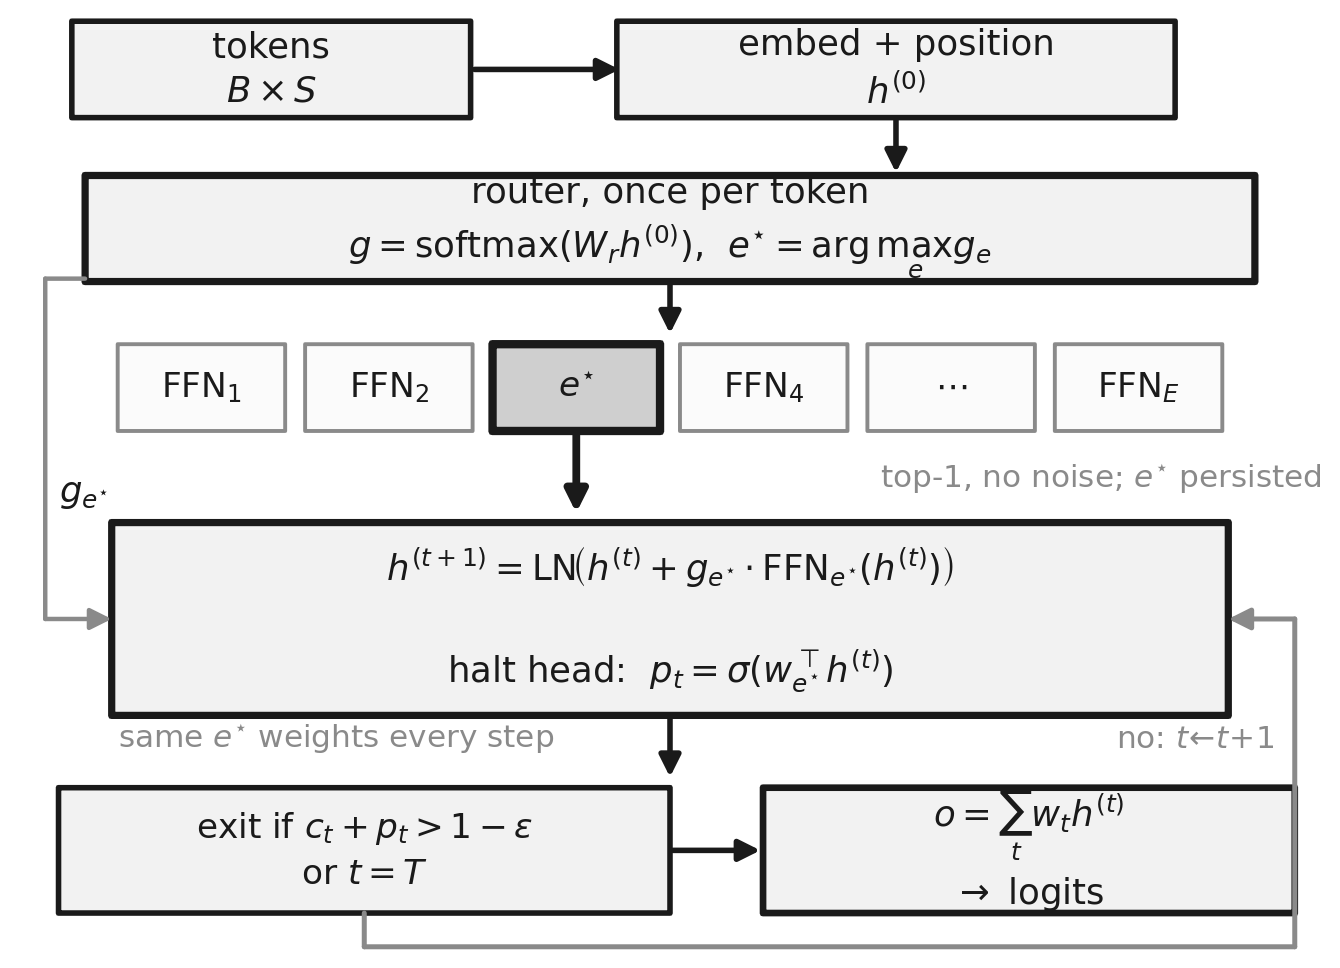
\includegraphics[width=\linewidth,keepaspectratio]{fig_architecture.png}
    \caption{The MoRE block. A token is routed \emph{once} to one of $E$
    independent expert FFNs; that experts weights are then reused for an
    adaptive number of recursion steps under ACT halting. Setting $T=1$ recovers
    MoE exactly and setting $E=1$ recovers MoR; the input representation is
    bit-identical in all three cases.}
    \label{fig:architecture}
\end{figure}

\subsection{Halting and the training objective}
\label{sec:halting-method}

Halting follows ACT \citep{graves2016act} as used in the Universal Transformer,
with one halt head per expert. Per token, at step $t$:

% Narrow-column form: the three-column align with a cases block ran 55pt outside
% a 234pt column. Two columns, shorter case labels, epsilon stated in the prose.
\begin{align}
p_t &= \sigma\big(\mathbf{w}_{e^\star}^{\!\top}\mathbf{h}^{(t)}\big),
  \quad c_t = \textstyle\sum_{\tau \le t} p_\tau , \label{eq:halt-p} \\[2pt]
&\text{halt when } c_t + p_t > 1 - \epsilon , \label{eq:halt-cond} \\[2pt]
R &= 1 - c_t , \quad
  w_t = \begin{cases} p_t & \text{running} \\ R & \text{at halt} \end{cases}
  \label{eq:halt-w}
\end{align}
with $\epsilon = 0.01$ and $R$ the halting remainder.

and the token's output is the convex combination
$\mathbf{o}_s = \sum_t w_t \mathbf{h}^{(t)}$, whose weights sum to exactly $1$.
That sum-to-one property is the mechanism by which halting is trained: because
$w_t$ scales how much of each step's state reaches the output, changing $p_t$
changes the task loss, so a differentiable path runs from $\mathcal{L}_{\text{task}}$
into the halt parameters. The boolean comparison in
Eq.~\ref{eq:halt-cond} decides dispatch only. Tokens still active at $t=T$ are
forced out; halted states are frozen and not recomputed, so a halted token costs
nothing at deeper steps.

Depth is trained through the expected-depth term
\begin{equation}
\rho \;=\; \mathbb{E}_{\text{tokens}}\big[\,N + R\,\big],
\label{eq:ponder}
\end{equation}
where the step count $N$ is discrete and contributes no gradient while the
remainder $R$ does. Eq.~\ref{eq:ponder} is the ponder cost. It is worth noting
that the gradient reaching the halt heads through $R$ is small compared with the
task gradient: a direct measurement in our implementation puts the halt gradient
at roughly $285\times$ below the task term. This ratio is the quantitative form
of the failure analysed in \S\ref{sec:mechanism}: the ponder term is large enough
to be optimised away but too weak to hold depth down once the task gradient
accumulates, and once the halting sigmoid saturates the gradient through $R$
vanishes \citep{graves2016act}. \citet{banino2021pondernet} is the principled fix
and is future work (the Limitations section).

The training objective is a weighted sum of terms that we report separately and
never as a single number:
% Narrow-column form: five terms with underbrace annotations ran 65pt outside a
% 234pt column. Stacked, with the annotations moved into the prose below -- which
% already names the weight on each term, so nothing is lost.
\begin{equation}
\begin{aligned}
\mathcal{L} \;=\;& 1.0\,\mathcal{L}_{\text{task}}
   + 0.001\,\mathcal{L}_{\text{bal}} + 0.001\,\rho \\
  &+ 0.0\,\mathcal{L}_{\text{fam}} + 0.0\,\mathcal{L}_{\text{route}} .
\end{aligned}
\label{eq:loss}
\end{equation}
$\mathcal{L}_{\text{task}}$ is per-token cross-entropy in nats.
$\mathcal{L}_{\text{bal}} = -H(\bar{\mathbf{g}}) + E\sum_e f_e \bar{g}_e$ combines
a router-entropy bonus with the Switch-style auxiliary \citep{fedus2022switch},
where $f_e$ is the dispatched load fraction and $\bar{\mathbf{g}}$ the mean soft
router probability; it is averaged over the depth calls actually made, so its
magnitude does not grow with $T$. Three terms are structurally zero on language
and the reason is not convenience. $\mathcal{L}_{\text{fam}}$ reads
$\mathbf{h}.\mathrm{detach}()$, so its gradient cannot reach the trunk---which
\emph{strengthens} every specialisation claim below relative to a comparable
synthetic study, where a family cross-entropy is typically one of the larger terms
in the objective. $\mathcal{L}_{\text{route}}$ and the halting-supervision term are
zero because natural language supplies no per-token oracle expert and no per-token
oracle depth to supervise against. The canonical router is therefore unsupervised
with respect to the per-token routing decision.

\subsection{One engine, three modes}\label{sec:engine} MoE, MoR and MoRE are configurations of one implementation with an explicit \texttt{architecture} mode, so a difference between arms cannot be a difference in the harness. Equalising \emph{total} FFN hidden width gives MoR's single FFN a multiplier of $24=4\times6$: \textbf{5{,}584{,}908 parameters for MoE and MoRE, identical, and 5{,}581{,}063 for MoR}---a $0.069\%$ deficit that is the router MoR lacks, and which runs \emph{against} our headline since the lighter arm wins in domain. Appendix~\ref{app:engine} derives it.

\section{Experimental Setup}
\label{sec:setup}

\subsection{Data and split}
\label{sec:data}

All arms train on WikiText-103 \citep{merity2017wikitext} with a byte-pair
vocabulary of 8{,}192 tokens and packed sequences of length 256
% The literal identifier is 41 characters of \texttt, and TeX sets
% \hyphenchar to -1 for typewriter, so it cannot break anywhere and ran 98pt
% past the margin. Short phrase here, literal string in the appendix.
(identifier in Appendix~\ref{app:protocol}). We use the corpus's own
author-provided validation split rather than carving one out of the training
material, which is what makes the leakage audit in \S\ref{sec:integrity}
meaningful: no validation or test token was ever available to the trainer.

The baseline floor is a backoff bigram estimated on the same corpus:
\textbf{4.9849 nats/token} (7.19 bits, perplexity 146.2). A model that does not
beat it has learned nothing a two-column count table could not. All three arms
beat it, by margins of $+1.037$, $+1.470$ and $+1.348$ nats for MoE, MoR and MoRE
respectively.

\subsection{Training protocol}\label{sec:protocol} Five seeds per arm, reported as mean$\,\pm\,$std, with one optimiser configuration fixed before the comparison and \emph{not} swept per architecture. \textbf{Three epochs is a compute budget, not convergence}: one epoch is 134.7M tokens against $\approx$3.4M non-embedding parameters, so no arm is converged. Every arm gets the identical budget, so the comparison holds; the consequences are in the Limitations section. Appendix~\ref{app:protocol} gives the hyperparameters.
\subsection{Metrics}\label{sec:metrics} The primary metric is \textbf{validation task loss}, final-epoch per-token cross-entropy in nats; \texttt{best} equals \texttt{last} on all 15 cells, so \emph{no model selection occurred}. Routing is scored with permutation-invariant measures (AMI, Hungarian, purity) against a per-run shuffled-label control and reported as a z-score, since unsupervised expert indices carry no semantic identity. Depth is reported with its exit rates alongside, because a depth--difficulty correlation taken on an arm whose tokens almost all reach the ceiling is computed against a near-constant and \textbf{says nothing about allocation}. Appendix~\ref{app:metrics} defines each.
\subsection{Statistics}
\label{sec:stats}

Comparisons use an exact two-sided randomization test on the difference of means,
which enumerates every way of splitting the pooled values into groups of the
original sizes---$\binom{10}{5} = 252$ at five-versus-five---and counts the
fraction whose $|$mean difference$|$ is at least the observed one. It is
exhaustive, hence deterministic: no sampling error, no seed, no normality
assumption, and no threshold to choose. The superseded $k\times$std heuristic is
not used anywhere.

The \textbf{resolution floor} of this design --- the smallest $p$ it can return at
all --- is $2/\binom{n_a+n_b}{n_a}$ for equal arms, which is $2/252 = 0.00794$ at
five-versus-five. The factor of two is there because the two-sided statistic is
invariant under swapping the groups, so extreme regroupings arrive in mirror pairs
and the count at the extreme can never be one.
The derivation is in Appendix~\ref{app:floor}.
\textbf{Every headline comparison in this paper sits exactly on that floor}, which
we phrase as ``as extreme as a five-seed design admits''---a weaker statement than
significance, and not to be dressed up as a stronger one. Only more seeds can
strengthen these claims; no larger effect can.

The correction is Holm--Bonferroni over two pre-registered families (predictive quality, $m=4$; adaptive depth, $m=2$), declared before the final arm was trained. Appendix~\ref{app:stats} gives the family memberships and explains why plain Bonferroni would be unusable here.

\subsection{Integrity checks}\label{sec:integrity} Three invariants hold across the matrix, each machine-checked: inputs are bit-identical across arms per record; the target is absent from the input and no oracle routing label is encoded in a feature slot; and the arms are parameter-matched to 0.069\% with seed-blind configurations identical within each arm. Three loss terms are structurally zero on language, one of which \emph{strengthens} the specialisation claims. Appendix~\ref{app:integrity} gives each in full.

\section{Results}
\label{sec:results}

\subsection{Predictive quality}
\label{sec:quality}

Table~\ref{tab:main} is the headline. Recursion alone is lowest-loss. MoR beats
MoE by $0.4329$ nats and beats MoRE by $0.1216$. Both recursive arms beat MoE
decisively, and the composition lands between them---the premise that routing
would \emph{add} to recursion in domain is not supported.

\begin{table*}[t]
\centering
\small
\caption{Canonical results, 5 seeds each, mean$\,\pm\,$std. Primary metric is
final-epoch validation task loss; \emph{best} is the minimum over evaluated
epochs and equals \emph{last} on all 15 cells, so no model selection occurred.
$\Delta$ floor is the margin below the bigram baseline of 4.9849 nats
(positive \emph{beats} it). FLOPs are inference FLOPs/token at each arm's
measured mean depth, from the FLOP accounting described in \S\ref{sec:metrics}. Pairwise, on the
primary metric: MoRE$-$MoE $-0.3113$ ($d\,{-}15.9$, $p\,0.0079$); MoRE$-$MoR
$+0.1216$ ($d\,{+}4.7$, $p\,0.0079$); MoE$-$MoR $+0.4329$ ($d\,{+}14.7$,
$p\,0.0079$). Exact two-sided randomization test, floor $p_{\min} = 0.00794$;
every headline comparison sits on it.}
\label{tab:main}
\vspace{2pt}
\begin{tabular}{lrrrrrr}
\toprule
& Params & val task loss & PPL & $\Delta$ floor & FLOPs/tok & items/s \\
\midrule
MoE  & 5{,}584{,}908 & 3.9483\,$\pm$\,0.0242 & 51.9 & $+1.0366$ & 5.25\,M & 724 \\
MoR  & 5{,}581{,}063 & \textbf{3.5154\,$\pm$\,0.0340} & \textbf{33.6} & $+1.4695$ & 47.6\,M & 170 \\
MoRE & 5{,}584{,}908 & 3.6370\,$\pm$\,0.0134 & 38.0 & $+1.3480$ & 11.5\,M & 170 \\
\bottomrule
\end{tabular}
\end{table*}

Two features of the table deserve to be read together. First, MoE and MoRE are
parameter-\emph{identical} at 5{,}584{,}908 while MoR sits $0.069\%$ lower at
5{,}581{,}063, the residual being the router MoR does not have---and that residual
runs \emph{against} the headline, since the arm with fewer parameters is the one
that wins. Second, MoRE has by far the tightest seed spread, and the difference is real
rather than impressionistic: its variance is $6.4\times$ smaller than MoR's
($0.000179$ against $0.001155$; std $0.0134$ against $0.0340$), and an exact
one-sided permutation test on the variance ratio returns $p = 1/252 = 0.0040$,
which is that test's floor. \textbf{What the number means is still open.} The runs
that exist cannot separate a genuinely stabilising effect from the simpler account
that a model whose halting has collapsed to a near-constant has less left to vary
across seeds---and the second reading is the more parsimonious one. We report the
measurement and decline the interpretation. (Exploratory and uncorrected: the
variance comparison is outside both declared families.)

Fig.~\ref{fig:depth-curve} and the forced-depth sweep sharpen this. Both arms scale
with forced depth up to a point, in opposite directions:

\begin{itemize}[leftmargin=1.4em,itemsep=1.5pt,topsep=2pt]
\item \textbf{MoR} improves from 7.36 nats at depth 1 to a minimum of 4.06 at
  depth 4, then \emph{degrades} to 4.99 at depth 7. It has a genuine interior
  optimum.
\item \textbf{MoRE} improves monotonically all the way to depth 7 (3.70), never
  turning over within the budget. It wants more depth than it has.
\end{itemize}

\begin{figure*}[t]
\centering
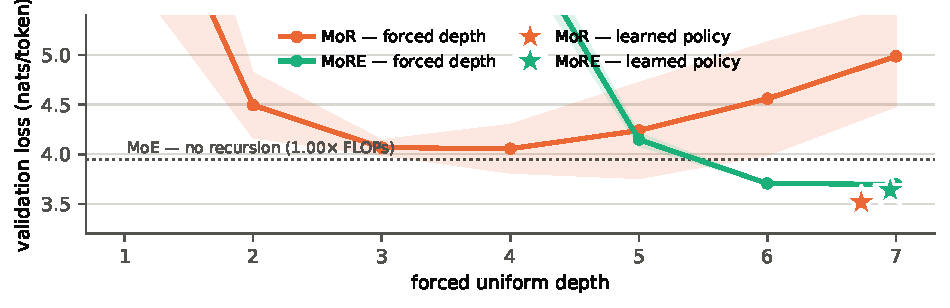
\includegraphics[width=0.92\linewidth]{fig_depth_curve.pdf}
\caption{Validation loss against forced uniform recursion depth, five seeds. Lines
are the forced-depth sweep; stars mark each arm's \emph{learned} policy at its own
measured mean depth. MoR's learned policy sits far below its own best uniform depth
(3.515 vs 4.056); MoRE's sits just below its forced-depth-7 endpoint (3.637 vs
3.697). The dotted line is MoE, which has no recursion. This is the paper's central
contrast: adaptive depth buys MoR a great deal and MoRE very little.}
\label{fig:depth-curve}
\end{figure*}

\subsection{Is recursion actually adaptive?}
\label{sec:halting}

The mechanism claim rests on comparing each learned policy against a \emph{uniform}
policy at the same compute, which is the cheapest competitor that ignores its input
and therefore the minimum bar an adaptive-depth claim must clear. Two comparisons
matter, and they give different answers for the two arms.

\textbf{Against the best uniform depth anywhere} (the strongest competitor): MoR's
learned policy at 3.5154 beats its best forced depth (4.0558 at $d{=}4$) by
\textbf{0.540 nats}. MoRE's learned policy at 3.6370 beats its best forced depth
(3.6971 at $d{=}7$) by \textbf{0.060 nats}.

\textbf{Against a depth-matched uniform policy}---forced to exactly the arm's own
measured mean depth of 6.955, so the comparison isolates \emph{where} the compute
goes rather than \emph{how much} there is: MoR's adaptive policy beats forced-$d7$
(4.9863) by \textbf{1.471 nats}; MoRE's beats forced-$d7$ (3.6971) by
\textbf{0.060 nats}.

The depth-matched comparison is the one that licenses a mechanism claim, because
best-depth comparison conflates adaptivity with the average compute spent. On it,
both arms' halting is doing something real and measurable---but MoR's buys 1.47
nats where MoRE's buys 0.06, a factor of roughly 24. The honest summary is not that
MoRE's depth mechanism is inert; it is that adding routing left it almost entirely
without effect.

\paragraph{The depth-matched control, as a general diagnostic.}
We state this separately because it generalises past this architecture and is, we
think, the most transferable thing in the paper. \textbf{A mean step count and an
exit histogram---the two statistics this literature almost always reports---do not
establish that depth depends on the input.} A policy that ignores its input
entirely can reproduce any mean and, with a little variance, a plausible-looking
histogram. The comparison that does establish input-dependence is against a
\emph{uniform policy forced to the learned policy's own mean depth}: it holds total
compute fixed, so the only thing left to differ is \emph{where} that compute was
spent. It costs one inference pass per checkpoint, needs no retraining, and it is
what separates our two arms---both of which look adaptive by mean-and-histogram,
and only one of which is. We recommend it as a routine check before any model is
described as allocating computation adaptively.

The exit statistics say why MoRE's margin is so small. MoR early-exits
$18.8\% \pm 15.1\%$ of validation tokens with mean depth $6.730$ and a halt
remainder of $0.175$; MoRE force-exits $97.3\% \pm 0.8\%$ at the ceiling with mean
depth $6.955$ and remainder $0.655$. MoRE's halting has collapsed to ``run to
budget''.

\textbf{The depth--difficulty correlation is reported next to those rates because
it is only interpretable alongside them.} MoR's per-token depth correlates with
per-token model loss at $\rho = +0.2985 \pm 0.0654$, positive on \textbf{5/5}
seeds. MoRE's is $-0.0230 \pm 0.0115$---but with $97.3\%$ of tokens exiting at the
ceiling and a per-token depth standard deviation of 0.43, that correlation is
computed against a near-constant. We report it as \emph{uninformative}, not as
evidence that MoRE allocates depth badly. This distinction is the paper's most
load-bearing methodological point: a near-zero correlation with a constant is not
a finding about allocation.

MoR's early-exit rate is the seed-unstable quantity ($6.4\%$--$42.2\%$ across
seeds), and its instability is informative. The two seeds that exit most are the
two with the \emph{worst} loss, and the three that exit least are the best. So the
\emph{alignment} of depth with difficulty is robust while the \emph{amount} of
compute skipped is seed-unstable and costs loss---which is why the mean is reported
with its standard deviation rather than as a single depth budget.

\subsection{Where the composition does pay: robustness and efficiency}
\label{sec:ood}

Out of domain the ordering inverts. Table~\ref{tab:evals} evaluates all three arms
on the same checkpoints, and scores each against the inference FLOPs it costs.

\begin{table*}[t]
\centering
\small
\caption{Evaluation battery, five seeds. Every cell is
\emph{score (difference vs MoE, inference FLOPs$\times$ vs MoE, $|$difference$|$
per FLOPs-multiplier)}. The \emph{score} is lower-better for loss rows and
higher-better for accuracy rows; the third number is a \textbf{modulus} and is
higher-better on \emph{every} row---it is how much quality each unit of compute
bought. The two axes are distinct and we never trade one for the other
rhetorically: columns 1--2 are quality at matched parameters, column 3 is quality
per unit of inference compute. \textbf{These are exploratory}: they sit outside
both declared families, are uncorrected, and carry no significance verdict.}
\label{tab:evals}
\vspace{2pt}
\begin{tabular}{llll}
\toprule
Eval & MoE & MoR & MoRE \\
\midrule
Val loss (nats) & 3.948 (1.00$\times$) & \textbf{3.515} ($-0.433$, 9.07$\times$, 0.048) & 3.637 ($-0.311$, 2.19$\times$, \textbf{0.142}) \\
Test loss (nats) & 3.947 (1.00$\times$) & \textbf{3.513} ($-0.435$, 9.07$\times$, 0.048) & 3.621 ($-0.326$, 2.19$\times$, \textbf{0.149}) \\
OOD loss (nats) & 8.272 (1.00$\times$) & 7.802 ($-0.470$, 9.07$\times$, 0.052) & \textbf{7.573} ($-0.699$, 2.19$\times$, \textbf{0.319}) \\
BLiMP (acc) & 56.63 (1.00$\times$) & \textbf{58.74} ($+2.11$, 9.07$\times$, 0.233) & 58.36 ($+1.73$, 2.19$\times$, \textbf{0.791}) \\
\bottomrule
\end{tabular}
\end{table*}

Three things follow.

\textbf{In domain, all three arms are on the frontier; out of domain, MoRE
dominates.} Fig.~\ref{fig:pareto} plots loss against inference compute. In domain
no arm Pareto-dominates another: MoE is cheapest, MoR is best, MoRE sits between
them, so MoRE's in-domain claim is a \emph{ratio}---the most quality per unit of
compute---and not a position the others fail to occupy. We are explicit about this
because the weaker reading is the one a reviewer should be able to check and find
already stated.

Out of domain the relationship changes in kind rather than degree. On held-out
Pile blocks \citep{gao2020pile} MoRE reaches 7.573 nats against MoR's 7.802 and
MoE's 8.272, at $2.19\times$ MoE's FLOPs against MoR's $9.07\times$---so MoRE is
both cheaper and better than MoR, and \textbf{MoR is Pareto-dominated}. Its
advantage over MoE is $0.699$ nats against MoR's $0.470$, i.e. MoRE captures
$149\%$ of MoR's out-of-domain gain against $72\%$ in domain. The in-domain
ordering inverts, and this is the one respect in which composing the two
mechanisms does something neither does alone.

\begin{figure*}[t]
\centering
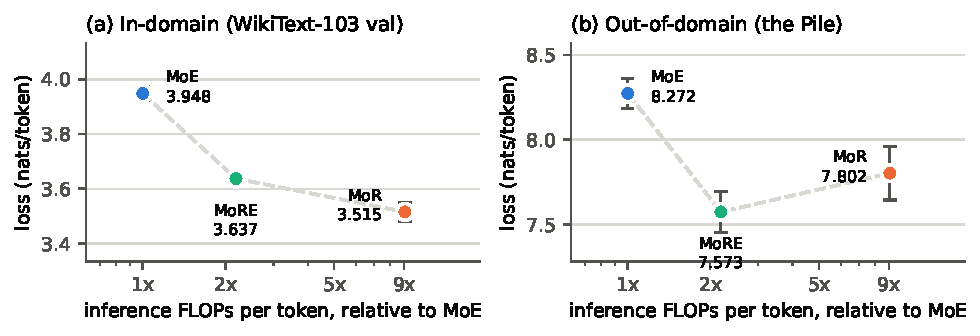
\includegraphics[width=0.98\linewidth]{fig_pareto.pdf}
\caption{Loss against inference FLOPs per token, five seeds, error bars one
standard deviation. (a) In domain no arm dominates another---the three trace a
frontier, and MoRE's claim is the slope from MoE, not its position. (b) Out of
domain MoR is \emph{dominated}: MoRE reaches lower loss at a quarter of the
inference compute. Exploratory, uncorrected.}
\label{fig:pareto}
\end{figure*}

\textbf{It gets there far more cheaply, on a different axis.} MoR attains the
lowest in-domain loss but pays $9.07\times$ MoE's inference FLOPs; MoRE pays
$2.19\times$, i.e. $24\%$ of MoR's total inference compute and $15\%$ of its
\emph{extra} compute over MoE. Per FLOPs-multiplier MoRE buys $0.142$ nats against
MoR's $0.048$---roughly $3\times$ the quality per unit compute on validation loss,
and $6\times$ on the out-of-domain row. \textbf{We state the two axes separately
and do not substitute one for the other}: at matched parameters MoR is lowest-loss
by $0.1216$ nats, which is significant at our resolution floor; per unit of
inference compute MoRE is ahead. ``Comparable to MoR'' is therefore only ever a
\emph{per-FLOP} statement in this paper, never an absolute-quality one.

FLOPs, not wall-clock, is the compute measure; the throughput column is reported so
the latency cost stays visible, and it shows MoRE no faster than MoR in wall-clock
(170 items/s each) despite doing $4\times$ less arithmetic, because its per-token
expert dispatch is latency-bound. An implementation that batches expert dispatch
would be expected to realise the FLOP advantage as wall-clock; ours does not, and
we do not claim a speedup.

\textbf{Grammatical competence is real but modest, and routing does not buy it.} On BLiMP \citep{warstadt2020blimp} both recursive arms beat MoE (58.74\% and 58.36\% against 56.63\%) and MoR is not distinguishable from MoRE ($p = 0.71$), so recursion buys measurable syntactic sensitivity and routing adds none. On EWoK \citep{ivanova2024ewok} all three arms sit at chance---a statement about scale, not architecture. Appendix~\ref{app:blimp} reports both.
\textbf{Both recursive arms gain most where prediction is hardest, and least where context is shortest.} Grouping validation loss by the frequency decile of the target token, the MoRE$-$MoE advantage grows from $-0.147$ nats on the most frequent decile to $-0.374$ on the rarest (MoR: $-0.188$ to $-0.527$), so neither gain is the uniform shift a pure capacity effect would produce. Grouping by position instead disconfirms the usual motivation for recursion: both arms gain most where context is \emph{longest}, not shortest. Appendix~\ref{app:stratified} gives both breakdowns.

\section{Why the Composition Fails}
\label{sec:mechanism}

Four accounts, labelled by evidential status: what is measured, and what is
hypothesis consistent with the measurement.

\subsection{Routing divides the data, not the update budget}
\label{sec:dilution}

\textbf{[Ordering MEASURED; arithmetic MEASURED; mechanism HYPOTHESIS.]} The
obvious account of the ordering is capacity dilution: MoR's single block sees
100\% of tokens while MoE and MoRE split the same FFN budget across six experts,
so each expert is trained less. \textbf{That account is arithmetically false
here, and ruling it out is what makes the surviving hypothesis worth stating.}

The budgets are matched by construction, and the matching cancels. Each MoE/MoRE
expert FFN holds $2 \cdot 4 \cdot d^2 = 524{,}288$ weights and MoR's single FFN
holds $2 \cdot 24 \cdot d^2 = 3{,}145{,}728$, exactly six times as many
(\S\ref{sec:engine}). A run sees $404.2$M tokens. So:

\begin{center}
\small
\begin{tabular}{lccc}
\toprule
per FFN parameter & MoE & MoR & MoRE \\
\midrule
tokens seen      & 128.5 & 128.5 & 128.5 \\
FFN applications & 128   & 865   & \textbf{894} \\
\bottomrule
\end{tabular}
\end{center}

Tokens per parameter is \emph{identical} across all three arms---the token split
and the parameter split are both by $E$, so they cancel exactly. And once
recursion is counted, applications per parameter slightly \emph{favours} MoRE
(894) over MoR (865), because MoRE runs marginally deeper. Whatever costs MoRE
0.12 nats against MoR, it is not that its parameters are trained less.

That comparison also explains the easy half of the ordering. MoRE gets
$894/128 \approx 7\times$ the FFN applications per parameter that MoE gets, which
is simply what recursion buys, and MoRE beats MoE by 0.311 nats. The recursive
multiply is real and it is the entire source of MoRE's advantage over MoE.

\textbf{What remains, once update count is excluded, is the \emph{diversity} of
what each parameter block sees.} MoR's block is exposed to the whole token
distribution; each MoE/MoRE expert is exposed only to the router-selected slice
that reaches it, which is both narrower and systematically biased, since the
router selects it. Structure shared across the whole distribution---the bulk of
what a language model must learn at this scale---can be learned once by MoR's
block but has to be re-learned independently inside all six experts. Six partial
copies of shared structure fit in the same parameter budget as one complete copy
only by making each copy worse.

This is a hypothesis, not an isolated effect, and we label it as one: separating
it from the remaining differences needs a width sweep or a controlled
manipulation of routing diversity, and we ran neither. It earns its place because
it is the only account left after the arithmetic above excludes the update-count
version, because it predicts the stratified result---MoRE's advantage over MoE
grows with token difficulty (\S\ref{sec:stratified}), which is where an
incompletely-learned shared structure should hurt most---and because it generates
the falsifiable scale prediction in the Limitations section: as the corpus grows,
each expert's slice eventually contains enough of the shared structure for the
re-learning penalty to amortise, so the MoR$-$MoRE gap should close with data
scale at fixed parameters.

\subsection{Depth saturation is a data-scale effect}\label{sec:saturation} \textbf{[MEASURED, four points at fixed hyperparameters.]} MoRE's halting sits at the ceiling on the full corpus (97.3\% forced-exit, mean depth 6.955 of 7), which invites the reading that the architecture cannot learn adaptive depth. A subset sweep falsifies that: at 2.5\%, 10\% and 40\% of the corpus the \emph{same} model at the \emph{same} ponder weight allocates depth adaptively---forced-exit rates near zero, mean depth between 1.9 and 2.4 inside a budget of 7---and the collapse appears only at full scale. \textbf{So the failure is a calibration finding, not an architectural one}: this ponder penalty cannot hold depth down at this corpus size. The subset axis is not cleanly monotone, so the honest phrasing is that saturation emerges somewhere between 40\% and 100\% of the data. The mechanism is consistent: the ponder term is linear in expected depth while the task gradient grows as the model fits, and once the halting sigmoid saturates its gradient vanishes \citep{graves2016act}. \citet{banino2021pondernet} is the principled fix; we did not run it. Appendix~\ref{app:saturation} gives the sweep.
\subsection{The two mechanisms compete for one budget}
\label{sec:competition}

\textbf{[MEASURED on a calibration grid; the canonical-corpus form is measured on
the balance axis.]} This is the paper's central claim, and it is the one that
explains why the composition does not merely fail to add but subtracts.

Depth and specialisation are not independent knobs in MoRE the way they are in MoR
and MoE separately. On the calibration grid, recovering adaptive depth by raising
the halting weight destroys expert differentiation:

\begin{center}
\begin{tabular}{lccc}
\toprule
halting weight & mean depth & AMI & val loss \\
\midrule
0.001 (frozen) & 2.698 & \textbf{0.2851} & 5.2352 \\
0.107 & 1.476 & \textbf{0.0025} & 5.3346 \\
0.500 & 1.072 & 0.0207 & 5.3306 \\
\bottomrule
\end{tabular}
\end{center}

AMI of 0.0025 is statistically indistinguishable from the shuffled-label control.
The mechanism is direct: fewer recursion steps means fewer expert applications per
token, which means fewer opportunities for experts to differentiate. \textbf{Tune
toward adaptive depth and specialisation collapses; preserve specialisation and
depth saturates.} Both mechanisms draw on the same per-token compute budget, and at
this parameter and data budget neither gets enough. (This grid is on a smaller dev
corpus at one seed; it is a mechanism demonstration and carries that caveat.)

The competition has a second face on the canonical corpus, along a different axis.
The routing balance term is load-bearing and cannot be traded away for depth
either: setting it to zero \emph{collapses} the expert load onto a single expert
(load entropy 0.0001) and drives AMI to zero. A near-uniform per-token router
distribution coexisting with balanced load and above-chance specialisation is
therefore not a pathology to be tuned out---and we note that we initially read it
as one before the sweep refuted us (the disclosures in the Limitations section).

Specialisation itself is real, and measured against per-run controls rather than
against chance. MoRE's AMI is $0.1803 \pm 0.0246$ against a permutation control of
$0.0249$, a controlled z of $13.43$; Hungarian-matched accuracy is $0.3592 \pm
0.0271$ against a control of $0.2464$. MoE's AMI is $0.1637 \pm 0.0478$ against a
control of $0.0364$ ($z = 6.82$), Hungarian $0.3616$ against $0.2966$. Both
six-expert arms find substantial above-chance structure---and, read together, the
two arms are not distinguishable from each other. Routing quality is approximately
the same with recursion as without it, which is the routing half of the
interference result: recursion does not improve routing, and routing does not
preserve adaptive depth, in the same architecture.

\textbf{We also tested, and falsified, the most attractive rival account.} Subspace trapping---that routing once confines a token to one expert and repeated application drives the state to a fixed point---predicts lower representational dimensionality, oscillating dynamics, and rescaling updates in the composed arm. All three predictions fail: participation ratio is \emph{higher} in the recursive arms (57.3 and 70.3 against MoE 41.5), velocity decays monotonically, and successive updates are near-orthogonal. Appendix~\ref{app:trapping} reports the three probes. Excluding it is what leaves the budget competition above as the account the data support.

\section{Conclusion}
\label{sec:conclusion}

We built the composition of sparse expert routing and adaptive recursion as a
single engine, held parameters and inputs fixed across its three configurations,
and measured what the combination buys at each level of inference compute. At
5.6M parameters on WikiText-103 it buys efficiency and robustness rather than
peak quality: all three arms lie on the quality/compute frontier, MoRE buys the
most quality per unit of compute ($7.9\%$ better than MoE at $2.19\times$ its
FLOPs, $72\%$ of recursion's gain for $24\%$ of recursion's compute), and out of
domain it \emph{dominates} recursion alone---lower loss at a quarter of the
compute, the one respect in which composing the mechanisms does something neither
does alone. What it does not buy is in-domain quality: recursion alone remains
lowest-loss by 0.1216 nats, significant at our resolution floor, and routing adds
nothing to routing quality over MoE either. We keep the two axes separate
throughout, and neither statement licenses the other.

The mechanism is not the obvious one. Routing does not dilute the update
budget---tokens per parameter are identical by construction---and the recursion
is not dynamically broken, since subspace trapping fails three ways. What the
evidence supports is a competition for one per-token budget: the arm that
preserves specialisation saturates its depth. We release the engine, the
evaluation battery, and the forced-depth control, and it is the last we would
most like to see reused. A mean step count and an exit histogram do not establish
that depth depends on the input---a policy ignoring its input reproduces
both---whereas scoring against a uniform policy forced to the same mean depth
does, costs one inference pass, and is what separates our two recursive arms by a
factor of 24. We recommend it as a routine check before any model is described as
allocating computation adaptively.


% ---------------------------------------------------------------------
% MANDATORY and page-limit-exempt, in this order: Limitations, then the
% optional Ethical Considerations, then references. Omitting Limitations
% is a desk rejection.
% ---------------------------------------------------------------------
\section*{Limitations}
\label{sec:limitations}
\label{page:limitations_start}

\subsection*{Scale, stated as a falsifiable prediction}

The study operates at 5.6M parameters, $d_{\text{model}} = 256$, one block, a
vocabulary of 8{,}192, and three epochs of WikiText-103. Sparse-MoE benefits are
known to emerge with scale, so a reviewer can reasonably say the negative result
may be an artefact of operating below the regime where sparsity pays. \textbf{That
objection is correct and cannot be answered with the runs that exist.}

Rather than hedge it, we convert it into the paper's forward claim. The account in
\S\ref{sec:dilution} is that routing divides the \emph{diversity} of data each
parameter block sees, not its update budget---which the arithmetic there shows is
matched exactly. That account predicts a specific crossover: as the corpus grows at
fixed parameters, each expert's router-selected slice comes to contain enough of
the distribution's shared structure that the re-learning penalty amortises, so
\textbf{the MoR$-$MoRE gap should narrow monotonically with training data and the
ordering should eventually invert in favour of the composition}. The out-of-domain
result (\S\ref{sec:ood}) is weak early evidence in this direction, since MoRE is
already the better arm on data it was not trained on.

The measurement that would falsify it: hold parameters, depth budget and optimiser
fixed; sweep training tokens over at least a decade; and report the MoR$-$MoRE gap
as a function of tokens per expert. If the gap is flat or widening, the diversity
account is wrong and the composition's deficit is structural. We did not run that
sweep, and a second model size---the single most valuable follow-up---is likewise
unrun.

\subsection*{Budget, not convergence}\label{sec:budget} The 3-epoch budget leaves every arm short of convergence (\S\ref{sec:protocol}), and the arms are furthest apart on that axis at the cutoff: the final-epoch drop is $0.091$ nats for MoE, $0.132$ for MoR and $0.176$ for MoRE, so \textbf{the arm that loses in domain is the one still improving fastest}. The ordering is budget-dependent in the direction this paper's mechanism predicts---a routing arm that re-learns shared structure more slowly (\S\ref{sec:dilution}) should be behind at a fixed budget and closing---and we do not extrapolate a crossing epoch, because the curves decelerate. Appendix~\ref{app:budget} gives the per-epoch curves and the rest of this section.

\subsection*{Statistical resolution}

$n = 5$ seeds puts every headline comparison exactly on the design's resolution
floor of $p = 0.00794$ (\S\ref{sec:stats}). ``As extreme as a five-seed design
admits'' is the strongest statement available, and it is weaker than significance.
No larger effect could produce a smaller $p$ here; only more seeds could. Cohen's
$d$ values are reported alongside every gap precisely because a large $d$ on a
small gap is the misreading to avoid---across our own re-exports, $d$ has moved by
a factor of 1.5 while the underlying gap moved by less than 0.005 nats.

\subsection*{What was declared and not run}
\label{sec:declared}

One comparison in the pre-registered Family A, a depth-matched fixed-depth control,
was declared before results existed and \emph{still consumes its Holm slot}: we do
not delete it to loosen the thresholds on the survivors. The forced-depth sweep in
\S\ref{sec:halting} answers the same question using inference passes over the
canonical checkpoints rather than a trained control arm, so we report it as an
exploratory mechanism result and leave the declared slot consumed and unfilled. A
fixed-depth sweep trained from scratch, a shuffled-depth control, and a
depth--input mutual-information analysis were all declared exploratory and are
unrun.

\subsection*{Evaluation caveats}

BLiMP and EWoK are scored with the tokenizer fitted to our training corpus
(8{,}192 BPE merges), so \textbf{absolute accuracies are not comparable to
published models} using 32k--50k vocabularies; only the cross-arm comparison is
valid. EWoK sits within noise of its 50\% chance floor for every arm, which we
report as a scale limitation rather than a result---at 5.6M parameters a world
knowledge probe is below its useful range. All evaluations outside the two declared
families are uncorrected and carry no significance verdict in the abstract or
conclusions.

The perplexities in Table~\ref{tab:main} are intra-study quantities for the same
reason and should not be compared to published WikiText-103 numbers.

\subsection*{Disclosures}
\label{sec:honesty}

% T-LA.24. The label and the subsection heading STAY in the body: four places
% cite the disclosures in the Limitations section (02_setup protocol line, 02_setup GPU sentence,
% 03_method ablation pointer, 05_mechanism trapping aside), and a label that
% moves to the appendix would silently re-point all four. Only the prose moves.
% The replacement keeps every integrity-critical fact at body length: the
% specification violation, the partial pre-registration, the GPU/revision split
% with its measured common-mode offset, and the depth-metric N/A.
\textbf{Disclosures.} Three facts count against this study and we state them plainly. An earlier composed arm re-routed at every step, violated the specification, and its apparent parity with MoR was an artefact---the architecturally correct arm scores $0.134$ nats \emph{worse}. The pre-registration is partial, and the MoR-versus-MoE comparison was specified after its data existed. And the matrix spans two GPUs over four code revisions; the retrained arms reproduced to $-0.117\sigma$ and $-0.119\sigma$, a common-mode offset that cancels in every between-arm gap carrying a verdict (the MoE$-$MoR gap moved by 0.000185 nats), though per-seed values do not reproduce and we do not claim they do. We likewise report no per-token depth-allocation error: English supplies no ground-truth depth, so the metric is \texttt{N/A}, not zero. Appendix~\ref{app:disclosures} gives all of it in full.


\section*{Ethical Considerations}
This work trains 5.6M-parameter language models on WikiText-103, a public corpus
derived from Wikipedia, and evaluates them on public benchmarks. No human
subjects, no annotation, and no personally identifying data are involved, and the
models produced are far below the scale at which generative misuse is a practical
concern. The realistic effect of the work runs through other researchers'
decisions rather than through deployment: we report a negative result about an
architecture combination, and a diagnostic---scoring any learned depth policy
against a depth-matched uniform policy before describing it as adaptive---that
should save compute otherwise spent on a mechanism that is not paying for itself.
The symmetric risk is that a null obtained at 5.6M parameters discourages work
that would succeed at scale; the Limitations section scopes the conclusion
for exactly that reason and states the measurement that would overturn it. The
corpus inherits the demographic and topical biases of Wikipedia, which we did not
measure and which bear on any downstream use of these checkpoints.

% acl.sty ALREADY issues \bibliographystyle{acl_natbib} (acl.sty:195), and the
% official ACL template calls only \bibliography. Declaring it again here put a
% SECOND \bibstyle into main.aux; bibtex answered "Illegal, another \bibstyle
% command", skipped the rest of it, and silently dropped one of seventeen
% citations -- with 0 LaTeX errors and nothing in the .log pointing at the cause.
% Do not add it back. (TMLR is the opposite case: tmlr.sty does NOT set it, so
% the TMLR main.tex must declare it.)
\bibliography{refs}

% ---------------------------------------------------------------------
% Appendices sit AFTER the references, keep the two-column format, and do
% not count toward the 8-page content limit. 08_appendix.tex is GENERATED
% by assemble_submissions.py from the ACLMOVE-marked blocks in the shared
% sources -- do not edit it here, it is overwritten on every rebuild.
% Reviewers are under no obligation to read it, so nothing load-bearing
% may live here: each block leaves a self-contained summary in the body.
% ---------------------------------------------------------------------
\appendix
% GENERATED by assemble_submissions.py -- do not edit.
% These blocks were lifted out of the body to meet ARR's 8-page
% content limit; appendices sit after the references and are exempt.

\section{The resolution floor of the randomization test}
\label{app:floor}

The argument is worth stating because the floor is a property of the design rather
than of the data. Our statistic is $|\mathrm{mean}(a) - \mathrm{mean}(b)|$. When
the two arms are the same size, the complement of any admissible group-$a$ subset
is itself an admissible group-$a$ subset, and swapping the groups negates the
difference while preserving its absolute value. Every regrouping at the observed
extreme therefore has a partner that is equally extreme, the count can never be
odd at the tail, and the smallest attainable fraction is $2/\binom{n_a+n_b}{n_a}$
rather than $1/\binom{n_a+n_b}{n_a}$. When the arms differ in size the complement
has the wrong size, is not an admissible regrouping, no mirror is forced, and
$1/\binom{n_a+n_b}{n_a}$ becomes attainable.

\section{Multiple-comparison correction}
\label{app:stats}

Correction is Holm--Bonferroni over two \emph{pre-registered} families, declared
before the final arm was trained: Family A (predictive quality, $m=4$, metric
validation task loss) and Family B (adaptive depth, $m=2$, metric depth--difficulty
correlation). The split is declared rather than chosen because the two families ask
different questions on different quantities, and pooling them would correct the
depth claim for tests that cannot bear on it. Holm controls the same familywise
error rate as plain Bonferroni and is uniformly more powerful, and here the choice
is load-bearing: plain Bonferroni over the seven comparisons would give
$0.05/7 = 0.00714$, \emph{below} the floor of 0.00794---a design in which no effect
of any size could be declared significant. Holm's easiest threshold at $m=4$ is
$0.0125$, a margin of 0.0046 above the floor.

Two consequences we hold ourselves to. A declared comparison that could not be run
still consumes its slot: dropping a failed arm must never make the survivors easier
to call significant. And a comparison whose floor exceeds its Holm threshold is
\emph{undecidable} and reported \texttt{N/A}, never ``not significant''---that
phrasing would blame the data for a limit of the design.

\section{Integrity checks and structurally-zero loss terms}
\label{app:integrity}

\subsection{Integrity checks}


Three mechanical invariants hold across the matrix, each enforced by an automated
check rather than by inspection. \textbf{(i) Inputs are bit-identical across arms
for the same record}: feature ranges are identical at $E \in \{1,5,6\}$, so a
difference between arms cannot be a difference in representation. \textbf{(ii) The
regression or classification target is absent from the input}, and no oracle routing
label is encoded into a feature slot. \textbf{(iii) The arms are parameter-matched
to 0.069\%} and the seed-blind configuration is identical within each arm, so
comparability cannot rest on a single code revision: the matrix spans four commits,
and it is the frozen specification plus the config-equality check that holds the
arms comparable, not one revision.

One disclosure belongs with the config table. Three loss terms are structurally
zero on language: the family-classification term because its head reads a detached
representation so its gradient cannot reach the trunk, and the routing-supervision
and halting-supervision terms because natural language supplies no per-token oracle
expert and no per-token oracle depth. The first is a genuine advantage over a
comparable synthetic study, where a family cross-entropy is often one of the larger
terms in the objective and every specialisation claim must be caveated for it.

\section{Loss stratified by token frequency and position}
\label{app:stratified}

\subsection{Stratified loss: the advantage concentrates on hard tokens}
\label{sec:stratified}

Fig.~\ref{fig:stratified} groups validation loss by the frequency decile of the
\emph{target} token---difficulty being a property of what must be predicted, not of
the input---and by position within the block.

Both recursive arms improve most where prediction is hardest. The MoRE$-$MoE
advantage grows from $-0.147$ nats on the most frequent decile to $-0.374$ on the
rarest; MoR's from $-0.188$ to $-0.527$. The widening is not monotone---the gap
dips at the seventh and tenth deciles---so we claim a trend, not a monotone
relationship. Neither architecture's gain is a uniform shift, which is what a
pure capacity effect would look like.

\begin{figure*}[t]
\centering
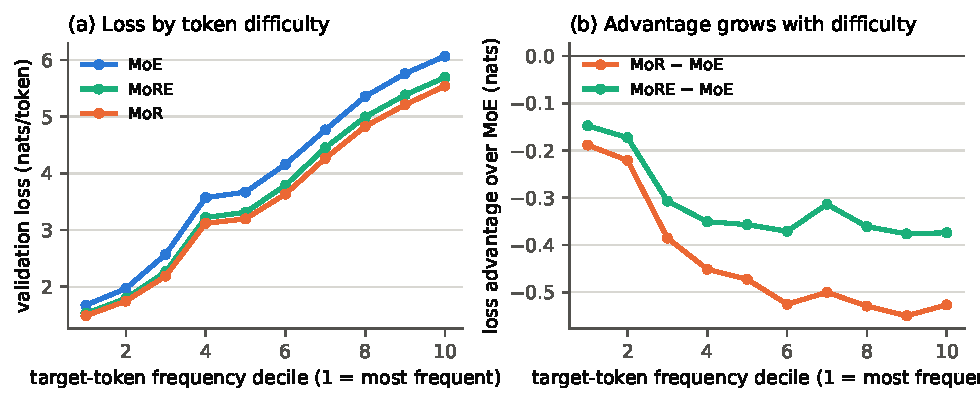
\includegraphics[width=0.98\linewidth]{fig_stratified.pdf}
\caption{(a) Validation loss by target-token frequency decile; decile 1 is the
\emph{most frequent} (easiest) and decile 10 the rarest. (b) Each recursive arm's
advantage over MoE, which widens toward the rarer deciles, though not monotonically.
Exploratory, uncorrected.}
\label{fig:stratified}
\end{figure*}

\textbf{A prediction this does not support.} If recursion were doing what the
adaptive-computation premise suggests---spending steps where context is thin---the
recursive arms should gain most at the \emph{start} of a block. They do the
opposite: MoRE's advantage over MoE is $-0.047$ nats in the first 8 positions and
$-0.359$ in the last 128; MoR's goes from $-0.250$ to $-0.465$. Both recursive arms
gain most where context is \emph{longest}. We report this because it disconfirms a
mechanism we would otherwise have asserted, and because it is consistent with the
capacity account in \S\ref{sec:mechanism}: a shared block iterated is accumulating
representation, not compensating for missing context.

\begin{figure*}[t]
\centering
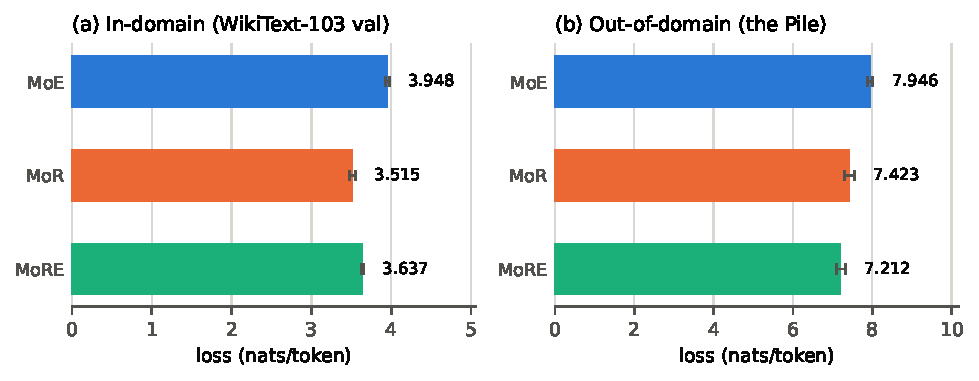
\includegraphics[width=0.98\linewidth]{fig_ood.pdf}
\caption{The ordering inverts out of domain: MoRE is worst in domain (a) and best
on the Pile (b). Same three entities and colours in both panels. Exploratory,
uncorrected.}
\label{fig:ood}
\end{figure*}

\section{The subspace-trapping probes}
\label{app:trapping}

\subsection{A plausible mechanism, refuted}
\label{sec:trapping}

\textbf{[MEASURED; hypothesis falsified.]} The natural explanation for MoRE's
collapse is \emph{subspace trapping}: routing a token once confines its recursion
to a single expert's parameter subspace, and repeated application of one block
within that subspace drives the state toward a fixed point rather than refining it.
It is an appealing account and it is wrong. We tested it three ways.

\begin{center}
\small
\begin{tabular}{lccc}
\toprule
probe & MoE & MoR & MoRE \\
\midrule
participation ratio    & 41.5 & \textbf{70.3} & 57.3 \\
inter-expert cosine    & 0.630 & \textsc{n/a} & 0.916 \\
\bottomrule
\end{tabular}
\end{center}
Participation ratio is the final-state value, $\pm$ 1.6, 5.6 and 2.8 across
seeds respectively; the cosine is the mean between-expert value.

\textbf{(i) Trapping predicts lower participation ratio in the composed arm;
it is higher.} If recursion were collapsing the state onto a low-dimensional
subspace, the composed model's final-state PR should fall below MoE's, since MoE
has no recursion at all. It does not: MoRE's PR is $57.3$ against MoE's $41.5$,
and MoR's---with no routing---is higher still at $70.3$. Recursion \emph{expands}
the effective dimensionality, and routing contracts it somewhat without collapsing
it. The ordering refutes the prediction.

\textbf{(ii) Trapping predicts oscillating or fixed-point dynamics; velocity
decays smoothly.} Measuring the L2 norm of consecutive post-norm states across
depth, both recursive arms decay monotonically---MoR from 11.06 at step 2 to 5.71
at step 7, MoRE from 9.09 to 3.49---which is the signature of settling, not of
vibrating around an attractor.

\textbf{(iii) Trapping predicts that successive updates rescale the state;
they are near-orthogonal.} The mean cosine between a step's update and the state
it updates from is negative in both arms ($-0.26$ to $-0.06$), i.e. updates push
into new directions rather than amplifying existing ones. A rescaling collapse
would show positive collinearity approaching $+1$.

The recursion in this architecture is dynamically healthy: it travels, it settles,
and it adds dimensions. The failure is not a broken iterated map. That rules out
the most attractive explanation and leaves the budget competition
(\S\ref{sec:competition}) as the account the data supports---which is a stronger
position than an unexplained null, because we can say which of the obvious
mechanisms it is \emph{not}.

\section{Matching the parameter budget across the three arms}
\label{app:engine}

\subsection{One engine, three modes}


MoE, MoR and MoRE are configurations of one implementation with an explicit
\texttt{architecture} mode, not three codebases. They share one data pipeline, one
optimiser setup and one evaluation path, so a difference between them cannot be a
difference in the harness. Only the fields their definitions require differ:
$E \in \{6,1,6\}$, $T \in \{1,7,7\}$, MoR's FFN multiplier (below), and the two
loss weights for quantities that do not exist in a given arm (no ponder cost at
depth 1, nothing to balance with one expert).

We write \textbf{MoR} for our recursion-only configuration---one shared block with
adaptive halting---which is in the spirit of weight-tied recursive transformers
with learned halting \citep{dehghani2019ut,bae2025mor} but is not a reproduction
of any specific published system; all three arms are configurations of the same
engine.

\paragraph{Matching the budget.} MoR has one FFN where MoRE has six, so matching
the per-FFN multiplier would compare 5.6M parameters against 0.9M and call the
difference architectural. We instead equalise \emph{total} FFN hidden width,
giving MoR's single FFN a multiplier of $24 = 4 \times 6$. The result is
5{,}584{,}908 parameters for MoE and MoRE, identical, and 5{,}581{,}063 for MoR---a
0.069\% deficit that is six per-expert halt heads, the router and FFN biases. That
residual is irreducible at any integer multiplier, and it runs \emph{against} the
headline result: the arm with slightly fewer parameters is the one that wins in
domain.

\section{Metric definitions}
\label{app:metrics}

\subsection{Metrics}


\textbf{Primary metric: validation task loss}, the final-epoch per-token
cross-entropy in nats. We deliberately do not select on best-epoch validation loss:
that is an order statistic whose downward bias scales with each arm's per-epoch
validation noise, which is not matched across architectures. On all 15 cells
\texttt{best} equals \texttt{last}---the evaluation interval is one epoch and the
curves decrease monotonically---so \emph{no model selection occurred} on either
split. Best-epoch values are reported alongside so the selection effect stays
checkable.

Because the router is unsupervised, expert indices carry no semantic identity, so
raw agreement with any externally defined partition measures label permutation as
much as partition quality. We therefore report AMI \citep{vinh2010ami},
Hungarian-matched accuracy and cluster purity, each against a \emph{per-run
permutation control}: the same metric computed against shuffled linguistic labels,
averaged over 10 draws. The controlled quantity is the z-score of the real value
against that null, not the raw value. The externally defined partition is a
part-of-speech hypothesis about a useful expert split---a hypothesis, not a
functional ground truth---so a router can be better for next-token prediction and
still score low against it. We therefore never call this ``routing accuracy''
without that qualifier.

For depth we report mean steps, exit rates, halt mass, and the Spearman correlation
between per-token depth and per-token difficulty. \textbf{The correlation is only
interpretable when depth has variance to correlate}: on an arm whose tokens almost
all exit at the ceiling, the correlation is computed against a near-constant and a
value near zero is uninformative rather than negative evidence. We report the exit
rates next to every correlation for that reason (\S\ref{sec:halting}).

\section{The subset sweep behind the depth-saturation finding}
\label{app:saturation}

\subsection{Depth saturation is a data-scale effect, not an architectural limit}


\textbf{[MEASURED, four points at fixed hyperparameters.]} MoRE's halting sits at
the ceiling on the full corpus (97.3\% forced-exit, mean depth 6.955 of 7). It is
tempting to read that as the architecture being unable to learn adaptive depth. A
subset sweep falsifies that reading.

\begin{center}
\small
\begin{tabular}{lcc}
\toprule
training data & mean depth & forced exit \\
\midrule
2.5\%             & 2.43 & $\approx 0$ \\
10\%              & 1.92 & $\approx 0$ \\
40\%              & 1.97 & $\approx 0$ \\
100\% (canonical) & 6.96 & 0.973 \\
\bottomrule
\end{tabular}
\end{center}

At every reduced-data point the same model, at the same ponder weight, allocates
depth adaptively---exit rates near zero, mean depth between 1.9 and 2.4, inside a
budget of 7. The collapse appears only at full scale. \textbf{So the failure is a
calibration finding, not an architectural one}: the ponder penalty that produces
adaptive depth on a small corpus cannot hold depth down at this one.

We state the limit of that claim precisely, because the sweep is exploratory
(single seed, subset fraction below 1, and it may never be quoted as a canonical
result). The subset axis is \emph{not} cleanly monotone---2.5\% gives 2.43 but 40\%
gives 1.97---so the honest phrasing is that \emph{saturation emerges somewhere
between 40\% and 100\% of the data}, not that depth is monotone in training steps.
The mechanism is consistent: the ponder term is linear in expected depth, while the
task gradient grows as the model fits, so the fixed penalty is outpaced. Once the
halting sigmoid saturates, its gradient vanishes and the linear-penalty ACT scheme
cannot recover on its own \citep{graves2016act}. \citet{banino2021pondernet}
replaces the linear penalty with a KL divergence against a geometric prior, which
keeps a gradient on the halt head near saturation, and is the principled fix; we
did not run it, and it is named as future work rather than as a result.

\section{Training protocol and hyperparameters}
\label{app:protocol}

\subsection{Training protocol}


% The ACL body replaced the 41-character dataset identifier with a pointer here,
% because \texttt cannot hyphenate and the literal string ran 98pt past the
% margin. It must therefore actually appear in the appendix. Nested inside the
% ACLMOVE:protocol block on purpose: the assembler resolves variants BEFORE
% extracting moves, so this lands in the ACL appendix and is absent from TMLR,
% which states the identifier in its own Data section.
The frozen dataset identifier is
\texttt{lang-\allowbreak wikitext-\allowbreak 103-\allowbreak bpe8192-\allowbreak len256-\allowbreak 800d6154}, and the split is the
corpus's own author-provided validation split.

Every canonical arm runs at seeds $\{42,43,44,45,46\}$ and is reported as
mean$\,\pm\,$std over five runs. Training is 3 epochs of AdamW (lr $10^{-3}$,
weight decay $10^{-4}$, gradient clipping 1.0, dropout 0.1) with
$d_{\text{model}} = 256$, one block, 4 attention heads, $T = 7$ and batch size 48
on a single laptop GPU. These settings were fixed once, before the comparison, and
not swept per architecture: they are a stable operating point, and no arm was tuned
for itself.

\textbf{Three epochs is a fixed compute budget, not convergence, and we state it
as such.} One epoch is 526{,}320 blocks $\times$ 256 tokens $= 134.7$M tokens
against $\approx$3.4M non-embedding parameters, so the runs sit in an underfitting
regime; the choice of 3 over 2 was made because the halting axis needs more than
two epochs to separate the arms at all, and going to 8 epochs was rejected on cost.
Every arm receives the identical budget, so the comparison is valid even though no
arm is converged. The consequences are stated in \S\ref{sec:limitations}.

\section{BLiMP and EWoK, in full}
\label{app:blimp}

\textbf{Grammatical competence is real but modest, and routing does not buy it.}
On BLiMP \citep{warstadt2020blimp}, 67{,}000 minimal pairs, both recursive arms beat
MoE (58.74\% and 58.36\% against 56.63\%) and MoR is not distinguishable from MoRE
($p = 0.71$). Every arm is above the 50\% floor, so recursion buys measurable
syntactic sensitivity at this scale; adding routing does not add more of it. The
gains concentrate on long-distance agreement phenomena---anaphor agreement and
determiner--noun agreement---which is where a shared iterative block would be
expected to help. We also ran EWoK \citep{ivanova2024ewok}, on which all three arms
sit within noise of the $50\%$ chance floor (49.62, 50.33, 49.95); that is a
statement about the scale of these models, not about the architectures, so we
exclude it from Table~\ref{tab:evals} and draw no comparison from it.



\end{document}
